\section{Data Prepossessing}
\label{se:data_preprocess}

The data imported via import modules may have incorrect data, missing data, and incompatible data which cannot directly feed into simulation modules.
Thus, we need to preprocess imported data before using them for weather forecasting. The WDIAS supports data preprocessing capabilities via extension modules. The current system has a few inbuilt extensions such as interpolation, transformation, and validation, but users can add more extensions as required.

\begin{figure}[htp]
    \centering
    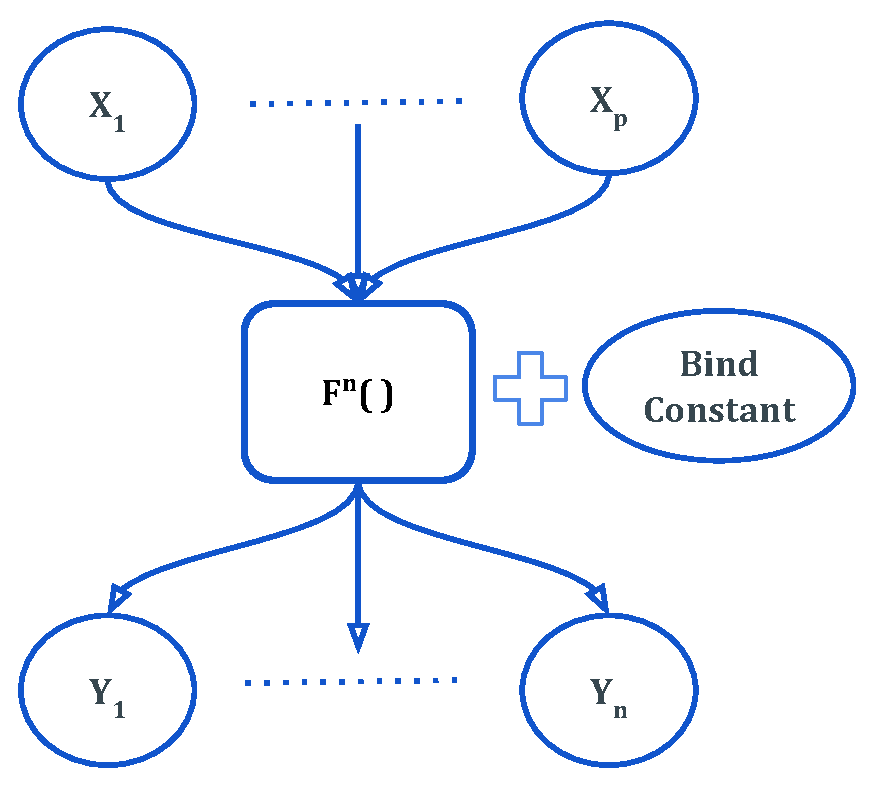
\includegraphics[width=0.6\textwidth]{method/data_preprocess/weather_data_preprocessing.pdf}
    \caption{A generic mathematical function model for weather data preprocessing.}
    \label{fi:weather_data_preprocessing}
\end{figure}

The data preprocess functionalities support simple generic mathematical function models. Each extension is considered as a mathematical function that can take \texttt{p} input timeseries variables and output \texttt{n} timeseries variables after applying the given function. Further, the system supports to provide a bind constant as configurations to the extension at the time of preprocessing. Thus, users can change the behavior of an existing function by providing different bind constants at the time of creating new triggers for an extension and produce different behaviors.

\subsection{Interpolation}
The interpolation module generates data at desired locations or desired data points using a serial or spatial interpolation technique. It is used to fill gaps in on-line measured data and to derive spatially distributed data for weather timeseries, such as precipitation and temperature, based on information available at nearby locations.

\subsubsection{Serial Interpolation}
During serial interpolation, we use interpolation to fill any gaps in a timeseries. The interpolation module will only consider a single timeseries, which is itself in filling these gaps.

\begin{figure}[htp]
    \centering
    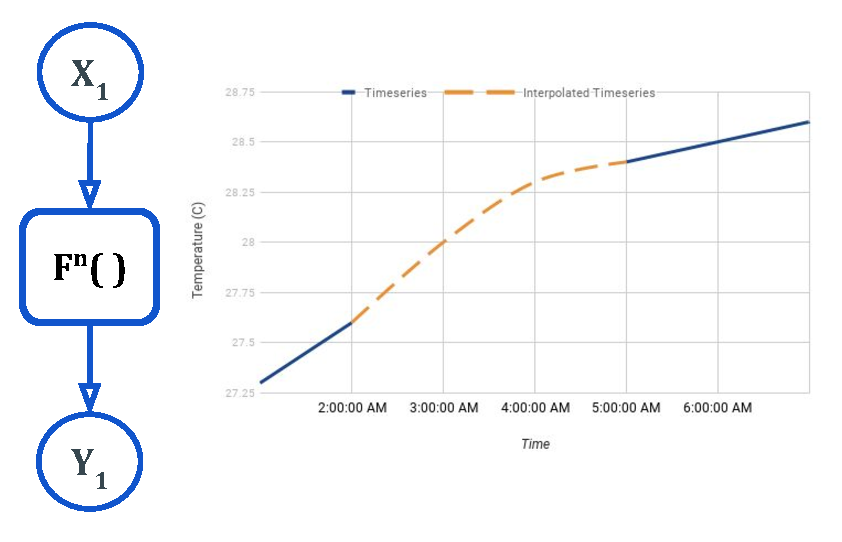
\includegraphics[width=1.0\textwidth]{method/data_preprocess/serial_interpolation.pdf}
    \caption{Serial interpolation.}
    \label{fi:serial_interpolation}
\end{figure}

\subsubsection{Spatial Interpolation}
During spatial interpolation, we use interpolation to either fill gaps in timeseries or to create a new timeseries for a location using data from other (spatially distributed) locations. Spatial interpolation can also be applied for sampling scalar timeseries from grid timeseries, for re-sampling grids, or for creating grids from timeseries data.
\begin{figure}[htp]
    \centering
    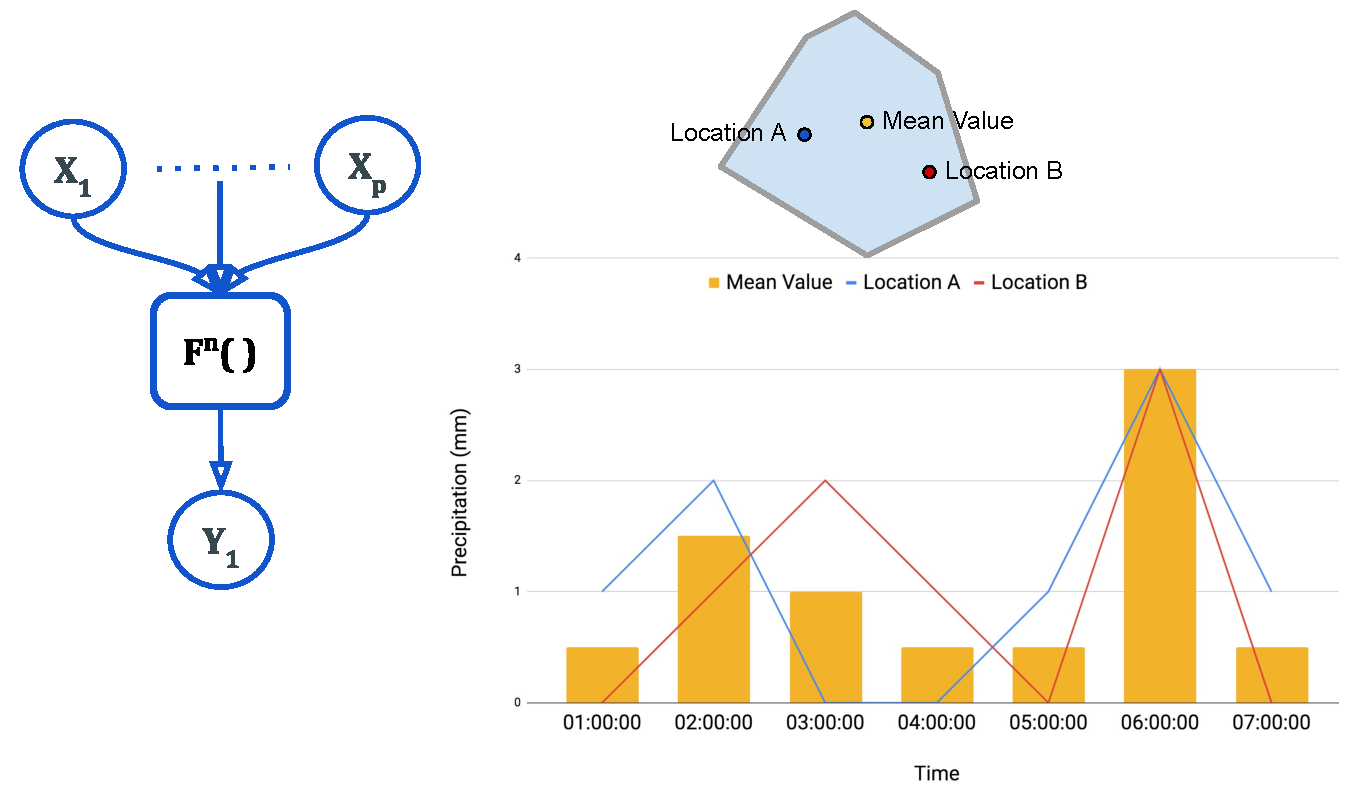
\includegraphics[width=1.0\textwidth]{method/data_preprocess/spatial_interpolation.pdf}
    \caption{Spatial interpolation.}
    \label{fi:spatial_interpolation}
\end{figure}

\subsection{Transformation}
Simple arithmetic manipulation of time interval transformation and shifting the series in time specific hydro-meteorological transformation such as stage discharge relationships.
\begin{figure}[htp]
    \centering
    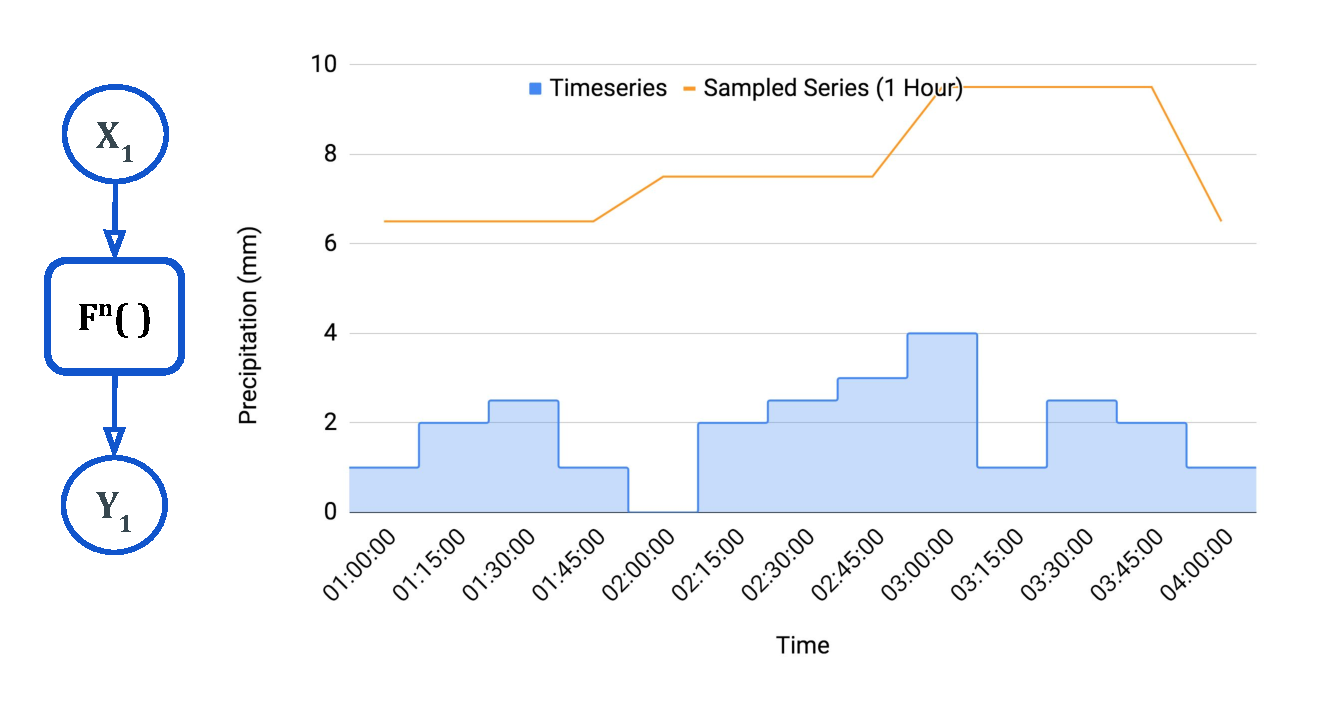
\includegraphics[width=1.0\textwidth]{method/data_preprocess/transformation.pdf}
    \caption{Time interval aggregration.}
    \label{fi:transformation}
\end{figure}

\subsection{Validation}
Checks for counting reliable, doubtful, unreliable, and missing values
\begin{figure}[htp]
    \centering
    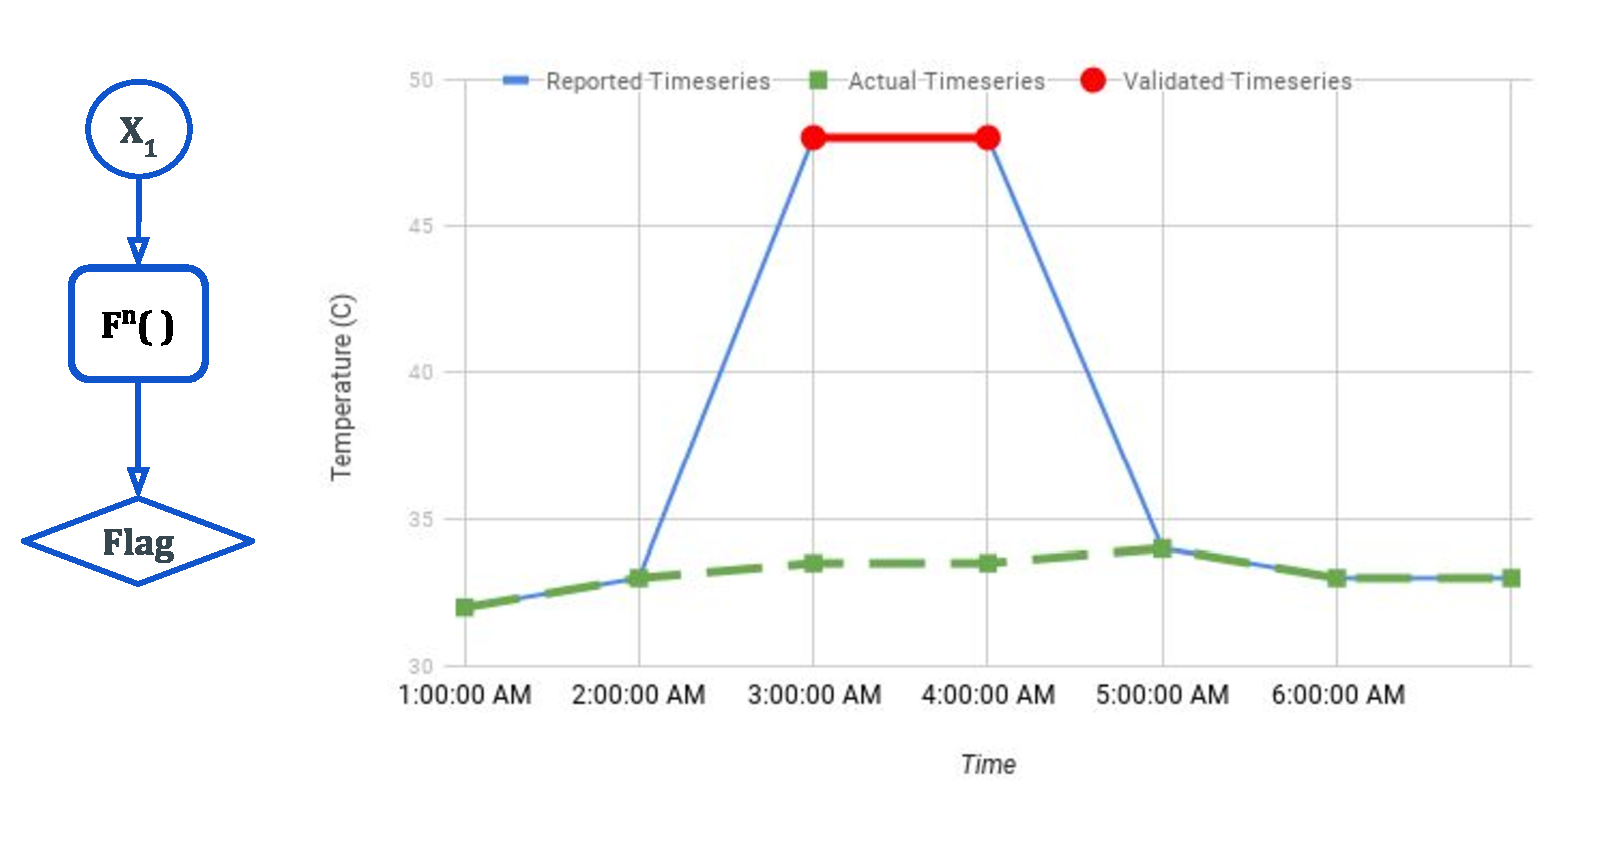
\includegraphics[width=1.0\textwidth]{method/data_preprocess/validation.pdf}
    \caption{Timeseries data validation.}
    \label{fi:validation}
\end{figure}

%%%%%%%%%%%%%%%%%%%%%%%%%%%%%%%%%%%%%%%%%%%%%%%%%%%%%%%%%%%%
\subsection{Extension API for Data Prepossessing}

We exposed an \acrshort{api} to create new triggers for extensions via /extension endpoint. Following is the accepted payload of the request while creating a new trigger. Later we discussed the \acrshort{api} in detail and how we can use the \acrshort{api} to create new triggers to use extension modules.

\begin{lstlisting}[language=Python]
{
    "extensionId": "",
    "extension": "Interpolation/Transformation/Validation",
    "function": "",
    "variables": [
        {
            "variableId": "",
            "metadata/metadtaIds": {
            }
        }
    ],
    "inputVariables": [],
    "outputVariables": [],
    "trigger": [
        {
            "trigger_type": "OnChange/OnTime",
            "trigger_on": []
        }
    ],
    "options": {
    }
}
\end{lstlisting}
\begin{itemize}
    \item \emph{extensionId} -- An unique identifier for new extension trigger. Should be unique among all extensions.
    \item \emph{extension} -- The main extension category which is responsible for handling the extension with extracting data required and storing the output. Interpolation/Transformation/Validation support for the moment.
    \item \emph{function} -- Name of the microservice which is handling the input to output mapping. \texttt{Fn()} function in the \cref{fi:weather_data_preprocessing}.
    \item \emph{variables} -- Array timeseries mapping to variables. Multiple variables can be define with metadata or metadataIds of timeseries. Can be use same variable on inputVariables and outputVariables below.
    \item \emph{inputVariables} -- Timeseries that need to be provide into the function.
    \item \emph{outputVariables} -- Timeseries that output from the function.
    \item \emph{trigger} -- Type of trigger for the extension. Should be one of OnTime or OnChange.
        \begin{itemize}
            \item \emph{OnChange}: \textit{trigger\_on} --- List of timeseries to listen on change and trigger the extension.
            \item \emph{OnTime}: \textit{trigger\_on} -- List of schedules that need to be trigger the extension in cronjob string format.
        \end{itemize}
    \item \emph{options} -- Bind Constant which is bind at the time of creating new extension trigger and pass on triggering the extension.
\end{itemize}

%%%%%%%%%%%%%%%%%%%%%%%%%%%%%%%%%%%%%%%%
\subsubsection{Extension Handler}

Extension handler is responsible for triggering the correct extension with timeseries metadata when there is any change in the subscribed timeseries which are provided as a list of \emph{OnChange} timeseries while creating an extension trigger.
When new data is imported into one of the scalar adapter or vector adapter, those microservices notify the extension handler. Then the extension-handler checks whether there is any extension subscribed for imported timeseries. If there is an extension needed to be triggered, then it invokes the given extension with the required data.

To improve the performance of matching triggers against a timeseries, we used two mechanisms as below. First, other than only storing extension metadata in a \acrshort{rdbms} instance of extension adapter, we also store extension data in a reverse lookup table called triggers while creating new extension triggers. Using this reverse lookup table, we can retrieve the extensions against a given timeseries without heavy processing and less delay. Second, we cache the resulting trigger type and timeseries metadata using the Redis database inside the extension handler for fast access and avoid too many queries on the \acrshort{rdbms} database. For the separation of service responsibilities, the extension data stored in the persistence database of the extension adapter and exposed via an endpoint.

%%%%%%%%%%%%%%%%%%%%%%%%%%%%%%%%%%%%%%
\subsection{Extension Scheduler}

Extension scheduler is responsible for triggering the correct extension with timeseries metadata at a given time that provided while creating an extension trigger as \emph{OnTime} cron job values. To improve the performance of triggering cron jobs at given time schedules, we used a few optimization mechanisms as described below. 
Same as for extension handler, the extension adapter exposed an endpoint to retrieve extension metadata grouped by cronjob time. Then we create cron jobs as per the data retrieved via extension adapter. We used a low-level programming language to simulate the cron jobs for fast processing the extensions. After getting extension triggers, the extension handler grouped them based on cronjob time and scheduled cron jobs programmatically to trigger at given times. 
When each cron job triggers at the scheduled time, each cron job also contains the extensions to be triggered. Fetching extension triggers data, and creating cron jobs occur with a long period to avoid huge overhead on extension adapter. When a user creates a new extension trigger, those data push into a queue in the Redis database. Then the extension handler pulls data from the queue in regular time intervals and creates new cron jobs for mentioned cronjob time. 
As mentioned above, to avoid the expansion of the programmatic cron job list that we created for new extension triggers, all cronjobs fetch again after a long period and flush the previously scheduled cron jobs. While doing that, we also flush the Redis queue.
The extension handler should be run as a single process for the atomicity, to avoid triggering the same extension twice.